\documentclass[12pt,a4paper]{article}
\usepackage[UTF8]{ctex}
\usepackage{amsmath,amssymb}
\usepackage{listings}
\usepackage{xcolor}
\usepackage{hyperref}
\usepackage{geometry}
\usepackage{graphicx}
\geometry{margin=2.5cm}

\lstdefinestyle{python}{
  language=Python,
  basicstyle=\ttfamily\small,
  keywordstyle=\color{blue}\bfseries,
  commentstyle=\color{gray},
  stringstyle=\color{red},
  showstringspaces=false,
  breaklines=true,
  frame=single,
  backgroundcolor=\color{gray!10}
}

\title{Quantum Monte Carlo / 量子蒙特卡洛}
\author{QuoNic}
\date{}

\begin{document}
\maketitle

\begin{center}
\textbf{Algorithms / 算法} | 难度：高级 | 预计时间：20 分钟
\end{center}

\tableofcontents
\newpage

\section{为什么需要？}

量子蒙特卡洛是经典蒙特卡洛方法的量子推广，提供二次加速。

\subsection{经典局限}
\b\begin{itemize}
  \item 经典蒙特卡洛需要 $O(1/\epsilon^2)$ 样本
  \item 对于高维积分，经典方法效率低
\end{itemize}

\subsection{量子优势}
\b\begin{itemize}
  \item 量子蒙特卡洛只需要 $O(1/\epsilon)$ 样本
  \item 提供二次加速
  \item 适用于高维积分和期望值估计
\end{itemize}

\subsection{实际应用}
\b\begin{itemize}
  \item 金融（期权定价）
  \item 物理（量子模拟）
  \item 机器学习（期望值估计）
\end{itemize}

\section{快速上手}

\begin{lstlisting}[style=python]
from quonic.algorithms import quantum_monte_carlo

# Estimate expectation value
result = quantum_monte_carlo(func="x^2", domain=[0, 1])
print(f"Estimate: {result.estimate}")
print(f"Error: {result.error}")
\end{lstlisting}

\textbf{预期输出}：
\begin{verbatim}
Estimate: 0.333
Error: 0.001
\end{verbatim}

\section{原理详解}

\subsection{电路图}

\begin{center}
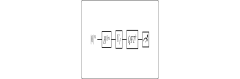
\includegraphics[width=0.7\textwidth]{../../images/quantum_monte_carlo_circuit.svg}
\end{center}

\subsection{数学推导}

量子蒙特卡洛估计积分：
\begin{equation}
I = \int f(x) p(x) dx
\end{equation}

\textbf{算法步骤}：
\begin{enumerate}
  \item 用量子态编码概率分布 $p(x)$
  \item 用受控门计算 $f(x)$
  \item 用 QPE 估计期望值
\end{enumerate}

\textbf{复杂度}：
\begin{equation}
O(1/\epsilon) \text{ vs } O(1/\epsilon^2)
\end{equation}

\subsection{几何解释}

量子蒙特卡洛利用量子叠加态同时采样多个点，通过干涉效应加速积分估计。

\section{代码详解}

\begin{lstlisting}[style=python]
from quonic.algorithms import quantum_monte_carlo

# quantum_monte_carlo(func, domain, shots)
# func: function to integrate
# domain: integration domain
# shots: number of measurements
result = quantum_monte_carlo(func="x^2", domain=[0, 1], shots=1024)

# result.estimate: estimated integral
# result.error: estimation error
print(f"Estimate: {result.estimate}")
\end{lstlisting}

\section{进阶用法}

\subsection{场景 1：不同函数}

\begin{lstlisting}[style=python]
# Different functions
result1 = quantum_monte_carlo(func="x^2", domain=[0, 1])
result2 = quantum_monte_carlo(func="sin(x)", domain=[0, 3.14])
result3 = quantum_monte_carlo(func="exp(-x^2)", domain=[-5, 5])
\end{lstlisting}

\section{适用场景}

\subsection{金融}

量子蒙特卡洛可以用于期权定价和风险分析。

\subsection{物理}

量子蒙特卡洛可以用于量子模拟和统计物理。

\section{常见问题}

\subsection{量子蒙特卡洛的加速比是多少？}

二次加速：$O(1/\epsilon)$ vs $O(1/\epsilon^2)$。

\subsection{量子蒙特卡洛的局限性是什么？}

需要能够高效编码概率分布和函数。

\section{学习路径}

\subsection{前置知识}
\b\begin{itemize}
  \item 量子相位估计
  \item 蒙特卡洛方法
  \item 概率论
\end{itemize}

\subsection{继续学习}
\b\begin{itemize}
  \item 量子金融
  \item 量子模拟
  \item 量子机器学习
\end{itemize}

\section{完整示例代码}

\subsection{示例 1：基本量子蒙特卡洛}

\begin{lstlisting}[style=python]
from quonic.algorithms import quantum_monte_carlo

result = quantum_monte_carlo(func="x^2", domain=[0, 1])
print(f"Estimate: {result.estimate}")
\end{lstlisting}


\section{下载}

\begin{itemize}
  \item [quantum_monte_carlo.py](https://github.com/ChrisLee0721/QuoNic/blob/main/examples/quantum_monte_carlo/quantum_monte_carlo.py)
\end{itemize}

\end{document}
